\documentclass[tikz,border=10pt]{standalone}
\usepackage{amsmath}
\usetikzlibrary{calc}
\begin{document}
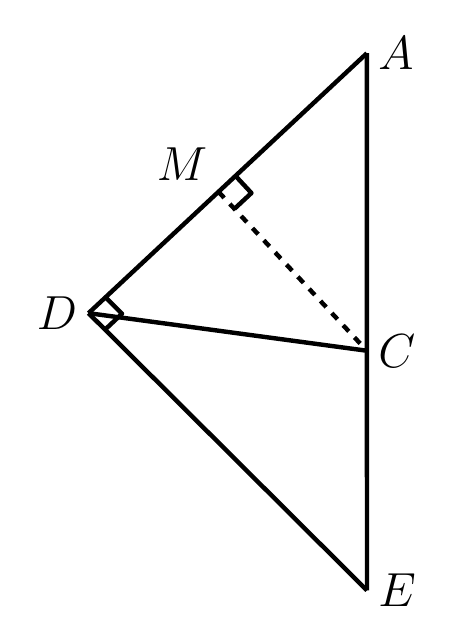
\begin{tikzpicture}[line width=1.6pt, line join=round]
  % Scale s = 0.01995 cm per px; y flipped about 446 px
  \coordinate (A) at (4.6559410455388175,7.8792631511417515);
  \coordinate (E) at (4.657540789721752,1.0571426871882088);
  \coordinate (D) at (1.1209266479387896,4.577952578946212);
  \coordinate (C) at (4.656827035546806,4.100952450691394);
  \coordinate (M) at (2.4330951515090766,6.493126348861796);
  % Foot F of the perpendicular from C onto AD (start of dashed segment)
  \coordinate (F) at (2.771669329744758,6.119562783170638);

  % Right-angle mark at F (existing, verified)
  \coordinate (P1) at (2.98812691817321,6.321073552678407);
  \coordinate (P2) at (3.1900114119803735,6.103967592932554);
  \coordinate (P3) at (2.973553823551921,5.902456823424783);

  % Right-angle mark at D between rays D->A and D->E (same 14.8 px square)
  \coordinate (Q1) at (1.3373848003230877,4.779463953552886);
  \coordinate (Q2) at (1.5466446338344952,4.571723300482648);
  \coordinate (Q3) at (1.331187722496893,4.36921317545303);

  % Solid segments
  \draw (A) -- (E);
  \draw (E) -- (D);
  \draw (A) -- (D);
  \draw (D) -- (C);

  % Dashed segment from foot F to C
  \draw[dashed] (F) -- (C);

  % Right-angle marks (one per right_angle object)
  \draw (P1) -- (P2) -- (P3);
  \draw (Q1) -- (Q2) -- (Q3);

  % Labels
  \node[right] at (A) {\fontsize{16}{19.2}\selectfont $A$};
  \node[right] at (E) {\fontsize{16}{19.2}\selectfont $E$};
  \node[left]  at (D) {\fontsize{16}{19.2}\selectfont $D$};
  \node[right] at (C) {\fontsize{16}{19.2}\selectfont $C$};
  \node[above left] at (F) {\fontsize{16}{19.2}\selectfont $M$};
\end{tikzpicture}
\end{document}
% GEOAGENT_REPAIR_V1 c18a466396f54661 2c714c6b7533afe2185bcea4860be87b24174c5cee331f0e6b65627939c30820
